%%%%%%%%%%%%%%%%%%%%%%%%%%%%%%%%%%%%%%%%%%%%%%%%%%%%%%%%%%%%%%%%%
% Contents: The importexport chapter
% $Id: grisbi-manuel-QIF.tex, v 0.4 2002/10/27 Daniel Cartron
% $Id: grisbi-manuel-QIF.tex, v 0.5.0 2004/06/01 Loic Breilloux
% $Id: grisbi-manuel-QIF.tex, v 0.6.0 2011/11/17 Jean-Luc Duflot
% $Id: grisbi-manuel-QIF.tex, v 0.8.9 2012/04/27 Jean-Luc Duflot
% $Id: grisbi-manuel-QIF.tex, v 1.0 2014/02/12 Jean-Luc Duflot
% $Id: grisbi-manuel-importexport.tex, v 3.0 2025/09 Dominique Brochard
%%%%%%%%%%%%%%%%%%%%%%%%%%%%%%%%%%%%%%%%%%%%%%%%%%%%%%%%%%%%%%%%%


\chapter{Importing and exporting accounts\label{importexport}}
%\chapter{Import et export de comptes\label{importexport}}

You can not directly use data that has been created by other personal accounting applications in Grisbi, and vice versa. Because these applications work differently, their data is structured differently, so you need to convert their data structure before you can use it.
%Vous ne pouvez pas utiliser directement dans Grisbi des données qui ont été créées par d'autres applications de comptabilité personnelle, et réciproquement. Comme ces applications fonctionnent différemment, leurs données sont structurées différemment: il faut donc convertir leur structure de données avant de pouvoir les utiliser. 

This conversion can not be done at once on all data, but must be done separately for each account managed by the application. To convert each of these accounts, you must first \enquote{export} them from the original application and then \enquote{import} them into the destination application.
%Cette conversion ne peut pas se faire d'un seul coup sur l'ensemble des données, mais doit se faire indépendamment pour chaque compte géré par l'application. Pour convertir chacun de ces comptes, il faut donc d'une part les \frquote{exporter} de l'application d'origine, puis les \frquote{importer} dans l'application de destination.

% espace avant Attention ou Note : 5 mm
\vspacepdf{5mm}

\Note{}: do not confuse the Grisbi file, with the \gls{extension} \file{.gsb}, which contains all the data of all the accounts created for the management of an accounting entity, and the \enquote{account files}, which are files that contain only data from one account at a time, and created only to export or import that data from one accounting application to another. These \enquote{account files} must have a \gls{file format} (or \gls{extension}) that must be compatible with the original application AND the destination application.
%\Note{}: ne pas confondre le fichier Grisbi, d'\gls{extension} \file{.gsb} et qui contient tous les comptes avec leurs données, et les fichiers de ces mêmes comptes, qui sont des fichiers ne contenant que les données d'un seul compte à la fois, et créés uniquement pour importer ou exporter ces données d'une application de comptabilité à une autre. Ces fichiers de compte doivent avoir un \gls{format de fichier} (ou une \gls{extension}) obligatoirement compatible avec l'application d'origine ET l'application de destination.


 %ne pas confondre LE \frquote{fichier de comptes} qui contient toutes les données de tous les comptes créés pour la gestion d'une entité comptable (dans Grisbi, ce fichier porte l'\gls{extension} \file{.gsb}), et LES \frquote{fichiers de compte}, qui sont des fichiers ne contenant que les données d'un seul compte à la fois, et créés uniquement pour exporter ou importer ces données d'une application de comptabilité à une autre. Ces \frquote{fichiers de compte} doivent avoir un \gls{format de fichier} (ou une extension) obligatoirement compatible avec l'application d'origine ET l'application de destination.
% espace après Attention ou Note : 5 mm
\vspacepdf{5mm}

Grisbi currently supports \gls{Gnucash}, \gls{OFX}, \gls{CSV} and \gls{QIF} personal accounting data formats.
%Grisbi supporte actuellement les formats de données de compte de comptabilité personnelle \gls{Gnucash}, \gls{OFX}, \gls{CSV} et \gls{QIF}.


\section{Importing accounts from another accounting application\label{importexport-import}}
%\section{Import de comptes d'un autre logiciel\label{importexport-import}}


If you want to use account data that has been created in another accounting application in Grisbi, you must first export each of the accounts of this application individually to a set of files, then import these same files into Grisbi.
%Si vous voulez utiliser dans Grisbi des données de comptes qui ont été créés dans une autre application de comptabilité, vous devez d'abord exporter individuellement chacun des comptes de cette application dans un fichier, puis les importer dans Grisbi grâce à ces fichiers.


\subsection{Export an account file from the other accounting application\label{importexport-import-exportinit}}
%\subsection{Export d'un compte d'un autre logiciel\label{importexport-import-exportinit}}

The first step is, in the originating personal accounting application, to export each account in a file in the chosen format. The chosen format must be compatible with the export formats supported by the original application \emph{and} compatible with import to Grisbi.
%La première étape consiste, dans l'application de comptabilité personnelle d'origine, à exporter chaque compte dans un fichier au format choisi. Le format choisi doit être compatible à l'exportation par l'application d'origine \emph{et} compatible à l'importation par Grisbi.

The export procedure is obviously different for each accounting application, so refer to its documentation. If you want to export all accounts, you will need to get as many files as you have accounts managed by the application.
%La procédure d'exportation est bien évidemment différente pour chaque logiciel, donc référez-vous à sa documentation. Si vous voulez exporter tous les comptes, vous devrez obtenir autant de fichiers que vous avez de comptes gérés par l'application.


\subsection{Importing account files from another accounting application to Grisbi\label{importexport-import-importinit}}
%\subsection{Import de fichiers de compte d'un autre logiciel dans Grisbi\label{importexport-import-importinit}}

\Note{}: Grisbi allows you to import one or more account files in one operation. Although you can import the account files one by one, it is important to import all the account files at the same time, so that Grisbi can recreate the links between the accounts, especially with regard to the transfer operations.
%\Note{}: Grisbi permet d'importer un ou plusieurs fichiers de compte au cours de la même procédure. Bien que l'on puisse importer les fichiers de compte un par un, il est important de bien importer tous les fichiers de compte simultanément, afin que Grisbi puisse recréer les liens entre les comptes, particulièrement en ce qui concerne les opérations de virement.
% espace après Attention ou Note : 5 mm
\vspacepdf{5mm}

For more information on the \indexword{account types}\index{account types} that Grisbi can manage, see the \vref{accounts-type}, \menus{Grisbi account types} section.
%Pour plus de renseignements sur les \indexword{types de compte}\index{types de compte} que Grisbi sait gérer, voir la section \vref{accounts-type}, \menus{Types de comptes de Grisbi}.

You can define which date will be used for assigning a financial year to each imported operation, see \vref{setup-general-import-financialyear}, \menus{Definition of Financial Year}.
%Vous pouvez définir quelle date sera utilisée pour l'attribution d'un exercice à chaque opération importée, voir le paragraphe \vref{setup-general-import-financialyear}, \menus{Définition de l'exercice}.

When you import a file, Grisbi allows you to establish an association between a string of characters in this file and a payee. For example, all labels containing \enquote{rent} may be associated with a payee that represents your landlord. This must be configured in the \menus{Edit - Preferences} menu (see the \vref{setup-general-importLinks}, \menus{Associations for Import} section).
%Lorsque vous importez un fichier, Grisbi vous permet d'établir une association entre une chaîne de caractères de ce fichier et un tiers. Par exemple, tous les libellés contenant \frquote{loyer} peuvent être associés à un tiers qui représente votre propriétaire. Cela doit être configuré dans le menu \menus{Édition - Préférences} (voir la section \vref{setup-general-importLinks}, \menus{Associations pour l'import}).

% espace pour changement de thème
\vspacepdf{5mm}
In the Grisbi \menus{File} menu, choose the option \menus{Import file} (or use the shortcut \keys{Ctrl+I}), which opens the import wizard window. The import of the account files takes place in five steps, to which one step must be added for each additional account:
%Dans le menu \menus{Fichier} de Grisbi, choisissez l'option \menus{Importer un fichier} (ou utilisez le raccourci-clavier \keys{Ctrl+I}), ce qui ouvre la fenêtre de l'assistant d'importation. L'importation d'un seul fichier de compte se déroule en cinq étapes, auxquelles il faudra rajouter une étape par compte supplémentaire:

\begin{enumerate}
	\item Launches the import assistant (step 1/5): confirm with the \menus{Forward} button;
	%Accueil de l'assistant d'importation (étape 1/5): validez avec le bouton \menus{Suivant};
	\item Selection of the account files to import (step 2/5) \refimage{importexport-import-files-select-img}:
	%Sélection des fichiers de compte à importer (étape 2/5) \refimage{importexport-import-files-select-img}:	
		\begin{enumerate}
			\item click the button \menus{Add file to import...} button : a file manager window opens;
			%cliquez sur le bouton \menus{Ajouter un ou des fichiers...}: une fenêtre de gestionnaire de fichiers s'ouvre;
			\begin{figure}[htbp]
				\raggedleft
				%\begin{flushleft}
					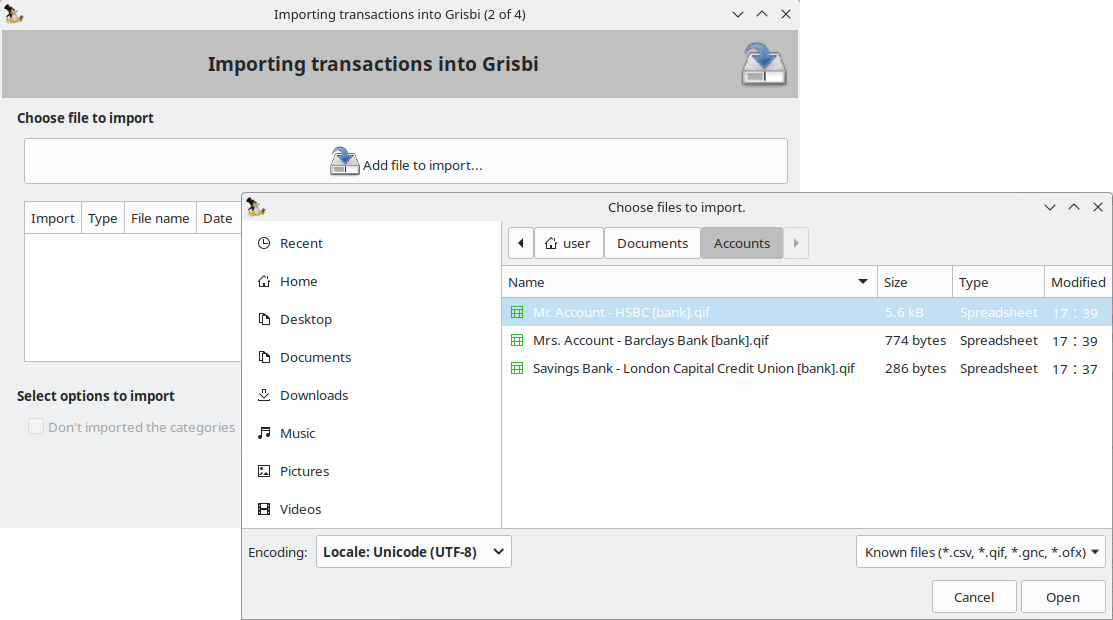
\includegraphics[width=.95\textwidth]{image/screenshot/importexport_import_files_select}
				%\end{flushleft}
				\caption{Selecting accounts to import}%Sélection des comptes à importer}
				\label{importexport-import-files-select-img}
			\end{figure}
			\item look for the directory where these account files are,
			%cherchez le répertoire où se trouvent ce ou ces fichiers de compte;
			\item select one or more account files (with the combination \keys{Ctrl+Left-Click} and \keys{Shift+Left-Click}); you can also change the \gls{locale} (\gls{character encoding}) of the files to import from the \menus{Encoding} drop-down menu,
			%sélectionnez un ou plusieurs fichiers de compte (avec la combinaison \keys{Ctrl+Clic Gauche} et \keys{Maj \shift+Clic gauche}); vous pouvez aussi changer la \gls{locale} (\gls{encodage des caracteres}) des fichiers à importer dans le menu déroulant \menus{Codage};
			\item validate the window with the \menus{Open} button to return to the account file selection window;
			%validez avec le bouton \menus{Ouvrir} pour revenir à la fenêtre de sélection des fichiers de compte;
			\item you can choose not to import categories by ticking the appropriate option. When importing a \gls{CSV} file, a new window allows you to choose the import settings \refimage{importexport-import-CSV-setup-img}:
			%vous pouvez choisir de ne pas importer les catégories en cochant l'option adéquate. Dans le cas d'import d'un fichier \gls{CSV}, une nouvelle fenêtre vous permet de choisir les paramètres d'import \refimage{importexport-import-CSV-setup-img}:
				\begin{itemize}[label=\textopenbullet]
					\begin{figure}[htbp]
						\raggedleft
						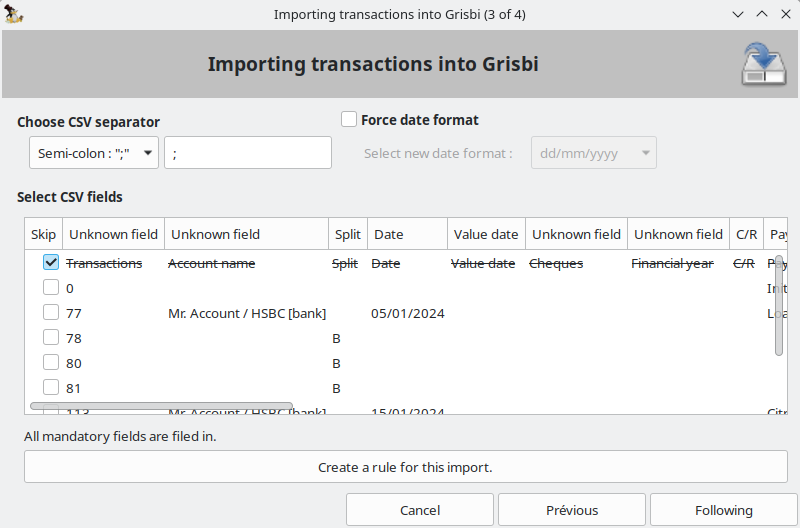
\includegraphics[width=.95\textwidth]{image/screenshot/importexport_import_CSV_setup}
						\caption{Configuring the import of a CSV file}%Paramétrage de l'import d'un fichier CSV}
						\label{importexport-import-CSV-setup-img}
					\end{figure}
					\item \textbf{Choose CSV separator}: the separator between data can be selected from the drop-down list in the left-hand window and is displayed in the right-hand window, where you can also modify it. 
					%\textbfChoisissez le séparateur CSV}: le séparateur entre les données peut être sélectionné dans la liste déroulante de la fenêtre de gauche et s'affiche dans la fenêtre de droite, où vous pourrez aussi le modifier;
					\item \textbf{Force date format}: The date format can be forced by ticking the appropriate box and selecting it from the drop-down list.
					%\textbf{Forcer le format de la date}: le format de date peut être forcé en cochant la case idoine et en le sélectionnant dans la liste déroulante;
					\item \textbf{Select CSV fields}: you can tick the data lines that \textit{will not be} imported;
					%\textbf{Sélectionnez les champs}: vous pourrez cocher les lignes de données qui \textit{ne seront pas} importées;
					\item The \enquote{Create a rule for this import.} button (at the bottom) allows you to create an import rule that you will need to name in order to validate it. You will find it in the account toolbar (see \vref{transactions-functions}).
					%le bouton \frquote{Créer une règle pour cet import.} (en bas) permet de créer une règle d'import que vous devrez nommer pour la valider. Vous la retrouverez dans la barre d'outils du compte (voir \vref{transactions-functions}).
				\end{itemize}
			\item when the desired files are checked, you can validate the selection with the \menus{Forward} button;
			%si les comptes choisis sont bien cochés, vous pouvez valider par le bouton \menus{Suivant};
		\end{enumerate}
	\item Complete the import of the account files (step 3/5): if everything went well, this window gives the list of the account files which will be imported; continue the import by confirming with the \menus{Forward} button;
	%Fin de la préparation de l'importation des fichiers de compte (étape 3/5): si tout s'est bien passé, cette fenêtre donne la liste des fichiers de compte qui seront importés; continuez l'importation en validant par le bouton \menus{Suivant};
	%TODO: FOLLOWING
	\item Création et paramétrage de chaque compte importé dans Grisbi (étape 4): vous pouvez passer en revue chaque compte et y choisir les actions suivantes	\refimage{importexport-import-files-setup-img}:
	\begin{figure}[htbp]
		\begin{center}
		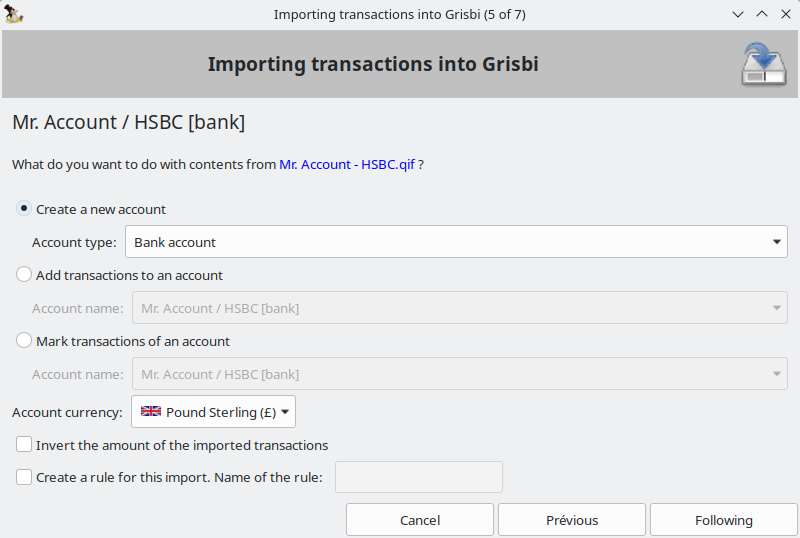
\includegraphics[width=0.95\textwidth]{image/screenshot/importexport_import_files_setup}
		\end{center}
		\caption{Paramétrage de chaque compte importé}
		\label{importexport-import-files-setup-img}
	\end{figure}
		\begin{itemize}
			\item \menus{Créer un nouveau compte}: cela ajoutera le fichier sélectionné comme nouveau compte dans votre fichier Grisbi. Le menu déroulant \menus{Type de compte}, en dessous, vous permettra de modifier le type de compte;
			\item \menus{Ajouter des opérations à un compte}: si des opérations planifiées sont trouvées dans l'intervalle de temps spécifié, une fenêtre spécifique s'ouvre pour savoir ce que vous voulez en faire: soit fusionner ces opérations planifiées avec les opérations importées correspondantes, soit ajouter les opérations importées en sus de celles-là (voir la section \vref{setup-general-import-parameters}, \menus{Paramètres pour l'import}). Le menu déroulant \menus{Nom du compte}, en dessous, vous permettra de sélectionner le compte auquel seront ajoutées les opérations;
			\item
			%\menus{Marquer les opérations d'un compte}: cela marquera les opérations avec un \frquote{T} dans la colonne \frquote{P/R} (\vref{transactions-list-fields}) du compte concerné. Si des \indexword{opérations orphelines}\index{opération!orpheline} sont trouvées, une fenêtre s'ouvrira en fin d'import pour savoir ce que vous voulez en faire: soit les ajouter, soit les ignorer. Le menu déroulant \menus{Nom du compte}, en dessous, vous permettra de sélectionner le compte dans lequel les opérations seront marquées;
			\item définir la devise du compte (ou bien en créer une nouvelle);
			\item \menus{Inverser le montant de l'opération importée}: utile pour les comptes de carte bancaire de la Banque Postale, par exemple;
			\item \menus{Créer une règle pour cet import}: permet de définir une règle d'import rapide si le fichier est au format \gls{QIF}, \gls{Gnucash} ou \gls{OFX} et uniquement si vous ajoutez ou marquez des opérations à un compte. Cette règle est spécifique à chaque compte et devra être nommée pour être validée. Vous pourrez la retrouver dans la barre d'outils du compte (voir \vref{transactions-functions});
			\item quand tout est correct, validez l'importation par le bouton \menus{Suivant};
		\end{itemize}
	\item Validation de la fin de l'importation: valider par le bouton \menus{Fermer}.
\end{enumerate}

Si, et seulement si, vous venez de créer votre fichier Grisbi juste avant cette importation de données de comptes, revenez à la fin de la section \vref{start-newfile-end}, \menus{Création d'un nouveau fichier de comptes}. Allez juste après la fin de la procédure de création du fichier de comptes, au paragraphe commençant par \textbf{\emph{D'une manière ou d'une autre\ldots{ }}}, ce qui vous proposera de créer tout de suite d'autres comptes.

%espace pour changement de thème
\vspacepdf{5mm}
Sinon, vous pouvez commencer à utiliser le compte que vous venez de créer.


\section{Export de comptes à partir de Grisbi\label{importexport-export}}


Si vous voulez utiliser, dans une autre application de comptabilité, des données de compte qui ont été créées par Grisbi, vous devez d'abord exporter ces données dans des fichiers, puis les importer dans l'autre application grâce à ces fichiers. Le format de fichier choisi doit être compatible à l'exportation par Grisbi \emph{et} compatible à l'importation par l'application de destination.
 
Dans le menu \menus{Fichier}, choisissez l'option \menus{Exporter vers un fichier QIF/CSV}  (ou utilisez le raccourci-clavier \keys{Ctrl+E}) qui ouvre l'assistant Export des comptes. L'exportation des comptes comporte à minima quatre étapes:

\begin{enumerate}
	\item Accueil de l'assistant (étape 1/3): cette fenêtre indique que, comme les formats de fichier \gls{QIF} et \gls{CSV} ne supportent pas les devises, toutes les opérations seront converties dans la devise de leur compte respectif; validez par le bouton \menus{Suivant};
	\item Sélection des comptes et des options \refimage{importexport-export-img}:
		\begin{figure}[htbp]
			\begin{center}
				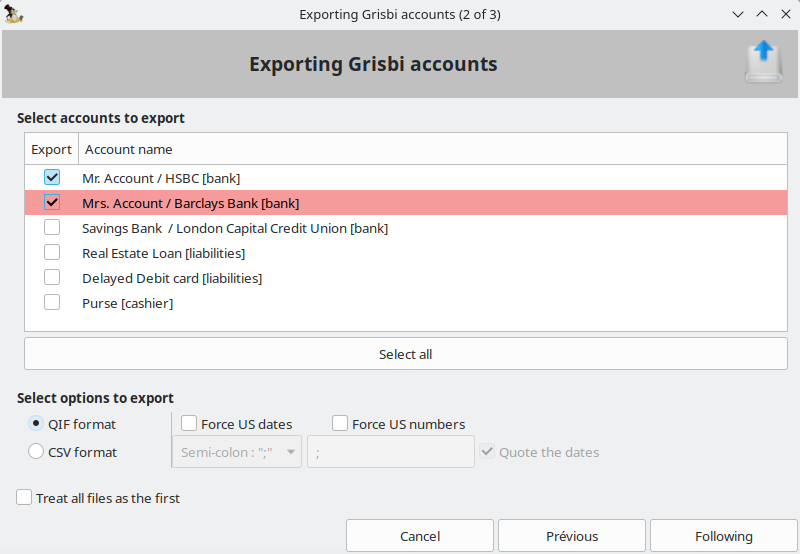
\includegraphics[width=0.95\textwidth]{image/screenshot/importexport_export}
			\end{center}
			\caption{Export des comptes}
			\label{importexport-export-img}
		\end{figure}
		\begin{itemize}
			\item \textbf{Sélectionner les comptes à exporter} (étape 2/3): cliquez sur la ou les cases correspondantes à chaque compte à exporter ou sur le bouton \menus{Sélectionner tout};
			\item \textbf{Sélectionner les options pour l'export}:
			\begin{itemize}
					\item \menus{Format QIF}: exporte le ou les comptes cochés au format \gls{QIF}; en plus l'option:
						\begin{itemize}
							\item
							%\menus{Force les dates au format US}: enregistre la date au format \frquote{mois/jour/année} (mm/dd/yyyy),
							\item
							%\menus{Force les nombres au format US}: utilise le point \frquote{.} comme séparateur de décimale et la virgule \frquote{,} comme séparateur des milliers;
						\end{itemize}
					\item \menus{Format CSV}: exporte le ou les comptes cochés au format \gls{CSV}; en plus des options disponibles au format QIF (ci-dessus):
						\begin{itemize}
							\item le séparateur entre les données peut être sélectionné dans la liste déroulante de la fenêtre de gauche et s'affiche dans la fenêtre de droite, où vous pourrez aussi le modifier;
							\item \menus{Citer les dates}: si cochée (par défaut), les dates seront mises entre guillemets, comme les autres données;
						\end{itemize}
			\end{itemize}
			\item \menus{Traiter tous les fichiers comme le premier}: ???;
			 validez par le bouton \menus{Suivant};
		\end{itemize}
	\item pour chaque compte, définissez le nom du fichier, le répertoire de destination et le format d'exportation, puis validez par le bouton \menus{Suivant}
	\item la fenêtre de fin de l'exportation s'affiche; validez par le bouton \menus{Fermer}.
\end{enumerate}

\Attention{}: d'une manière générale, il est déconseillé d'avoir des accents ou des espaces dans les noms des répertoires et fichiers utilisés par Grisbi. Si c'est le cas, renommez-les maintenant. Par exemple, les espaces peuvent être remplacées par des tirets bas (\_).